\documentclass[boldcaps,10pt]{USFDissertation}
%% Package options
% Font sizes (default 10pt)
%   10pt, 11pt, 12pt
% Headings styles (default plainheadings)
%   boldheadings (only bold), 
%   allcaps (chapter headings all caps only), 
%   boldcaps (bold and all caps), 
%   plainheadings (neither)

%% Keeping the preamble and title page in separate files keeps this one tidy

% Fill out the information that goes in the title page here
%% Fill out the title page

\title{Title Goes Here}
\author{Your Name}
\def\mydegree{The Degree You Want} % Doctor of Philosophy or Master of ___ (in ___)
\def\mydepartment{Mathematics \& Statistics} % or your department
\def\mycollege{Arts and Sciences} % or your college

% Comment out/delete anything you don't need

% One major professor
\def\mymajorprofessor{Major Professor, Ph.D.}

% OR two co-major professors
\def\mycomajorprofessorA{Co-Major Professor A, Ph.D.}
\def\mycomajorprofessorB{Co-Major Professor B, Ph.D.}

% Committee members
\def\mycommitteememberA{Committee Member A, Ph.D.}
\def\mycommitteememberB{Committee Member B, Ph.D.}
\def\mycommitteememberC{Committee Member C, Ph.D.}
\def\mycommitteememberD{Committee Member D, Ph.D.}
\def\mycommitteememberE{Committee Member E, Ph.D.}

% Key words should not be in the title
\def\mykeywords{buzz word, catchphrase, SEO}
\def\myapprovaldate{Month dd, yyyy} 
\def\mycopyrightdate{yyyy}

%% Feed author and title to hyperref metadata options. No need to do anything here.
\makeatletter
\let\theauthor\@author
\let\thetitle\@title
\makeatother

% The preamble.tex file is where you can load packages, define commands and macros. Some useful ones and templates are included already.
%% General use preamble. Some packages, environments, and macros are
%% included already as suggestions. Modify as needed.
\usepackage{mathtools}
\usepackage{amsmath, amsthm, amssymb, amsfonts, amsopn, bm, bbm}

% Silence warnings about \titlecap in hyperref links. This may silence other related warnings. Comment out to check.
\usepackage{silence}
\WarningFilter{hyperref}{Token not allowed in a PDF string}

% More flexibility formatting enumerated/itemized lists.
\usepackage{enumitem}

\usepackage{etoolbox} % General code fixing. Useful for macros that redefine things in the class file.

% To make pretty pictures with tex instead of importing figures. Comment out/delete if not drawing with pstricks. Be aware that adding a lot of images increases the time it takes to compile the document.
% Opacity does not work with PDFtex and you will have to change the compiler. On Overleaf, click on Menu - Compiler  and select XeLaTeX, 2020 version. The 2021 version has a bug that ignores opacity. Should be fixed in the 2022 version but that has not been released at time of writing (Summer 2022). 
\usepackage[usenames,dvipsnames]{pstricks}
\usepackage{epsfig}
\usepackage{pst-grad} % For gradients
\usepackage{pst-plot} % For axes
\usepackage[space]{grffile} % For spaces in paths

\usepackage{float}

\usepackage{relsize} % make large math symbols
\usepackage{tikz}
\usepackage{breqn} % break long math into lines

%%% Only loading these packages because this is a template. Not necessary for math, so feel free to delete this.
\usepackage{lipsum}

% With this you can insert pages from any other pdf document.
\usepackage{pdfpages}

% Modified list environment for a to-do list
\newlist{todolist}{itemize}{2}
\setlist[todolist]{label=$\square$}
% To include code that looks pretty
\usepackage{listings} % for code listing
\lstset{language=[LaTeX]TeX} % set the programming language for listings
\definecolor{codegreen}{rgb}{0,0.6,0}
\definecolor{codegray}{rgb}{0.5,0.5,0.5}
\definecolor{codepurple}{rgb}{0.58,0,0.82}
\definecolor{backcolour}{rgb}{0.95,0.95,0.92}
 
\lstdefinestyle{mystyle}{
    backgroundcolor=\color{backcolour},   
    commentstyle=\color{codegreen},
    keywordstyle=\color{magenta},
    numberstyle=\color{codegray},
    stringstyle=\color{codepurple},
    basicstyle=\ttfamily,
    breakatwhitespace=false,         
    breaklines=true,                 
    captionpos=b,                    
    keepspaces=true,                 
    showspaces=false,                
    showstringspaces=false,
    showtabs=false,                  
    tabsize=2
}
\lstset{style=mystyle}

\usepackage{printlen}
\usepackage{layout}
%%%%


%% Define theorem environments

% Use the syntax \newtheorem{<command>}[<counter>]{<Environment name>}

% Theorems are numbered by chapter, other environments use the same counter as theorems.
% If you change these commands, make sure to adjust the cleveref names below. 
\newtheorem{Thm}{Theorem}[chapter]
\newtheorem{Coro}[Thm]{Corollary}
\newtheorem{Prop}[Thm]{Proposition}
\newtheorem{Lem}[Thm]{Lemma}
\newtheorem{Conj}[Thm]{Conjecture}
\newtheorem{Prob}[Thm]{Problem}
\theoremstyle{definition}
\newtheorem{Def}[Thm]{Definition}
\newtheorem{Ex}[Thm]{Example}
\newtheorem{Rmk}[Thm]{Remark}
\newtheorem{Note}[Thm]{Notation}

% To add comments. Feel free to change the names/colors and add more people.
% Use syntax \Name{<text>}
\newcommand{\PersonA}[1]{{\color{OliveGreen}\textbf{Person A says:} #1}}

% A non-comprehensive list of useful math symbols, delimiters and operators.
% Hopefully enough examples are provided to help you write more of your own.
\newcommand{\N}{\mathbb{N}}
\newcommand{\Z}{\mathbb{Z}}
\newcommand{\R}{\mathbb{R}}
\newcommand{\tinfty}{\rightarrow \infty}
\newcommand{\seq}[1]{\left(#1_n\right)_{n \in \N}}
\DeclarePairedDelimiter\abs{\lvert}{\rvert}
\DeclarePairedDelimiter\ceil{\lceil}{\rceil}
\DeclarePairedDelimiter\floor{\lfloor}{\rfloor}
\DeclareMathOperator{\sign}{sign}

%% Some personalization can happen here. 

% For the bibliography
\usepackage[style=numeric,sortcites]{biblatex}
\addbibresource{biblio.bib}

% ETD guidelines suggest you can either indent all paragraphs or none. An argument can be made that paragraphs immediately after a section heading do not need to be indented* and this is the default LaTeX behavior. if you feel strongly about it, do not load the indentfirst package and talk to your ETD reviewer about your choice. At time of writing (Summer 2022), they seem to be willing to be lenient as long as the choices for indentation are consistent throughout the document. 

% *Chicago manual of style points out these are often flush left, and this appears to be a common choice among US/UK typographers, though it is not universal (MLA prefers ALL paragraphs without exception to be indented). You can choose your own (unless ETD reviewers are very insistent)

\usepackage{indentfirst}

\usepackage[dvipsnames]{xcolor}
\definecolor{pdflinkcolor}{rgb}{.1,.1,.6}	% darkblue
\definecolor{pdfcitecolor}{rgb}{.6,.1,.1}	% darkred
\definecolor{pdfanchorcolor}{rgb}{0,1,0}	% green
\definecolor{pdfurlcolor}{rgb}{.1,.6,.1}	% darkgreen
\definecolor{pdfpagecolor}{rgb}{0,0,1}	 % blue
\definecolor{pdffilecolor}{rgb}{1,0,0}	 % red

% Entirely optional, though it improves navigation for the readers of electronic documents. ETD guidelines at time of writing (Summer 2022) do not mention hyperlink formatting and reviewers seem to decide if they fit on a case by case basis. 
% If you are not attached (like I am) to hyperlinks, comment it out. If you want hyperlinks but want to avoid a round of formatting revisions, consider making all links black (i.e. citecolor=black,linkcolor=black, etc.). If you are determined, talk to ETD reviewers about your use of hyperlinks, they may let it slide.
\usepackage[%
breaklinks,
colorlinks=true,
citecolor=pdfcitecolor,
linkcolor=pdflinkcolor,
anchorcolor=pdfanchorcolor,
urlcolor=pdfurlcolor,
filecolor=pdffilecolor,
pagebackref=false,
pdfauthor={\theauthor},
pdftitle={\thetitle},
linktoc=page]{hyperref}

\usepackage[noabbrev,capitalize]{cleveref} % improvement

% Feeding the names of environments to cleveref. Adjust if needed.
\crefname{Thm}{theorem}{theorems}
\crefname{Prop}{proposition}{propositions}
\crefname{Lem}{lemma}{lemmas} % Lemmata for the extra pedanticc
\crefname{Coro}{corollary}{corollaries}
\crefname{Ex}{example}{examples}
\crefname{Rmk}{remark}{remarks}

%%%% Tidying up
% List of words that will not be capitalized in Title Case
\Addlcwords{of, and, a, an, the, or, to, in, on, at}

% Correct bad hyphenation here. Add words to the list separated by hyphens so that if LaTeX decides to break a line halfway through it does so correctly.
\hyphenation{hy-phen-a-tion}

%% Begin the document itself
\begin{document}

%% Make a title page
\maketitle

\doublespacing
% Dedication and acknowledgments
%% Maybe dedicate it to someone
\begin{dedication}
[Dedication placeholder]
\end{dedication}

%% Acknowledge your intellectual debts
\begin{acknowledgments}
[Acknowledgments placeholder]
\end{acknowledgments}

% Begin numbering with roman numerals
\frontmatter

\singlespacing
%% Insert a table of contents
\tableofcontents

%% Insert a table of tables -- comes before figures in the format.
% The tocloft package does not include a clear page, so we override that here.
\clearpage
\addcontentsline{toc}{chapter}{List of Tables}% Print LOT in TOC
\listoftables

%% Insert a table of figures
\clearpage
\addcontentsline{toc}{chapter}{List of Figures}% Print LOF in TOC
\listoffigures

\doublespacing
%% Include an abstract
\begin{abstract}
[Abstract placeholder]
\end{abstract}

%% Begin page numbering with arabic numerals
\mainmatter

%% Strongly suggest you make separate files for each chapter

%% Chapter 1
\chapter{Quick and dirty, a checklist}
More thorough explanations will follow, but if you're comfortable with \LaTeX and are ready to jump right in here's a TL;DR checklist to minimize the number of revisions ETD may suggest:

\begin{todolist}
\item Do you have a single major professor or two co-major professors? Make sure you use the correct settings in the title page and comment out what you don't need.
\item Scroll through the Contents and make sure everything looks right. 
\begin{todolist}
\item Chapter and section headings should use Title Case (where all words except some prepositions/articles are capitalized), and for subsections and lower levels, headings should use sentence case (regular capitalization). A package is currently adjusting all titles in chapters and sections to add title case, which should be reflected in the Table of Contents, but this may cause incorrect capitalization of some words.
\item Subsubsection headings should be in sentence case (only the first word and proper nouns are capitalized.) The Table of Contents only lists up to subsubsections but if you use any finer sectioning commands you will have to check that the headings printed correctly ``manually.''
\item Only the first sentence of each caption should appear in the List of Tables and List of Figures.
\end{todolist}
\item Especially if you copied and pasted the bibliography entries, double check that in the output file everything looks right and adjust as needed.
\item Though most widow/orphan lines should be taken care of, look out for orphan headings: headings (where the title prints) of subsections appear as the last line of a page. Fix these by adding \verb|\newpage| wherever appropriate.
\item Check the margins and make sure you don't have anything running off the sides of the page. When including long expressions in math mode in a paragraph, consider using \verb|\begin{sloppypar}| and \verb|\end{sloppypar}| to make sure they don't exceed the text width. 
\item If you have a lot of large images, they may leave large gaps in the text if you use \texttt{[H]} or \texttt{[h!]} positions. Relax them to \texttt{[h]} or even \texttt{[htpb]} so that large gaps, whenever appropriate, are filled with text. The guidelines say not to leave half a page or 5.5 inches empty, but shorter empty spaces will still be flagged by reviewers (because they're not measuring and neither are we). 
\item Equation environments, especially if you have large elementes like matrices, can be tricky because they look like images to the average ETD reviewer. It is easier (though not very elegant) to add/remove text where you can to make sure you're not leaving large empty spaces when equations happen near a page break.
\item Figures should have captions {\em below} and tables should have captions {\em above}. The space has already been assigned but you have to make sure to call the \verb|\caption| command in the right place. Scan through your document to make sure all captions are where they should be.
\item ETD reviewers will not check for content errors or typos, so comb through the document multiple times and make peace with the fact that you will almost certainly miss something. Just try not to let anything major slip through. 
\end{todolist}


%% Chapter 2
\chapter{How to use this template}
The goal of this template is to save you time (and effort) trying to put together your dissertation (hard enough as it is). This chapter covers many of the basics. 

\section{Overview}
This template uses multiple files to separate out chapters and major components as well as folders to neatly separate images. If this does not make your life easier, feel free to merge things later. All examples and instructions here assume the standard set up.

\begin{enumerate}
\item \texttt{titlepage.tex}. Fill this one out with all the relevant information for the title page. Make sure to comment out or delete anything you don't need. 
\item \texttt{preamble.tex}. You can load any additional packages you need here as well as create your own commands and macros. Some are already defined for you. 
\item \texttt{style_preamble.tex}. This one is for formatting nerds. Most things are handled by the .cls file, but you can a few things here without breaking anything (hopefully). 
\begin{itemize}
\item You can format the bibliography. Initially it is set to sort numerically. If you'd like to change the name used for the bibliography (currently set to ``References'') adjust it in the options of \verb|\printbibliography| on \texttt{main.tex}.
\item The \LaTeX default is to indent almost every paragraph (all {\em except} for paragraphs immediatelly after a heading). If you would rather indent {\em every} paragraph, without exception, remove the \% symbol to load the \texttt{indentfirst} package.
\item If you like to use hyperlinks, the \texttt{hyperref} package is loaded for you and initialized with {\color{pdflinkcolor}dark blue} (pdf links), {\color{pdfcitecolor}dark red}, and {\color{pdfurlcolor}dark green} for references. As of Summer 2022, the ETD guidelines do not mention hyperlinks so there is no established standard for whether or not to use them or how to implement them. You may conceal links by setting all colors to black, or disable them altogether by just not loading the \texttt{hyperref} package.
\item The \texttt{cleveref} package is loaded to make references a bit easier (examples of how later on). As far as formatting goes, just know that if you create new environments they may not get referenced correctly until you feed \texttt{cleveref} the correct names.
\end{itemize}
\item \texttt{dedication.tex} You can (optionally) dedicate your dissertation to anyone and write acknowledgments here. 
\item \texttt{abstract.tex} Self-explanatory, for the abstract.
\item \texttt{chapter<n>.tex} Only two of these are included but add as many as you like. Just make sure to lead with \verb|\chapter{<title>}| on the first line of each file.
\item \texttt{appendix.tex} After the \verb|\appendix| command is called, any additional chpaters are treated as an appendix. You can choose to include them all in one file (if they are short) or as separate files (\texttt{appendix01.tex, appendix02.tex}, etc.)
\item \texttt{biblio.bib} Feel free to modify this if \texttt{biblatex} is not your thing, but the default is to load it in the .cls file (be aware in case you load something else) and refer to the \texttt{biblio.bib} file for information. You can usually download citations in .bib format and then modify the entries so they are easier to cite. 
\item \texttt{main.tex} Not a lot happens here. To keep things tidy, you can add new files with \verb|\input{<filename>}| commands.
\end{enumerate}

\section{Quick start}
Just a few things to keep in mind as you write things. 
\subsection{Chapter headings}
Chapter headings can be modified by loading different options for the document class in \texttt{main.tex}.

\lstinputlisting[firstline=1, lastline=1]{main.tex}

The option \texttt{boldcaps} most closely resembles the sample .pdf files posted on the ETD website (as of Summer 2022), though \texttt{boldheadings} should also be acceptable. For the boldface averse, there are also \texttt{allcaps} (which uses all caps headings for chapters) and \texttt{plainheadings} (\verb|\normalfont| throughout), though they may not match guidelines. You can also modify the font size here. 

\subsection{title case and sentence case}
Chapter, section and subsection heading should use title case (Where Every Major Word is Capitalized), while everything else (subsubsection, paragraph, etc.) should use sentence case (Where only the first word and proper names are capitalized). Title case is implemented automatically. Note that while the title of this subsection is typed
\lstinputlisting[firstline=34, lastline=34]{chapter02.tex}
without any capital letters, it prints both in the heading and Table of Contents with correct capitalization. However, this setting does not affect subsubsections.

\subsubsection{title case is not applied here}
\subsubsection{You should use sentence case when typing titles}
The suggested use is to type all sectioning titles in {\em sentence case}. If it needs to be adjusted to title case, it will be done automatically and it will otherwise be left as is. The current settings in \texttt{USFDissertation.cls} are
\begin{lstlisting}
\usepackage{titlecaps} % For Title Case headings
% List of words that will not be capitalized in Title Case
\Addlcwords{of, and, a, an, the, or, to, in, on}
\end{lstlisting}
If any words that should remain lower case are incorrectly capitalized, add them there.

\section{Floats}
There is a very good chance you will have to include figures in your dissertation. Note that you can add an optional position parameter when you include floating elements. If you don't include any, \LaTeX will decide the placement for you. You can always force an element to appear exactly where it is called with \texttt{[H]} or \texttt{[h!]}, but be aware that it prevents any empty spaces after the object from being filled with text that is typed after it. The options for positions are 
\begin{itemize}
\item \texttt{h} Here. A soft suggestion.
\item \texttt{H} HERE. In shouty caps.
\item \texttt{t} Top, of the page.
\item \texttt{b} Bottom, self-explanatory.
\item \texttt{p} Page, meaning in a new page only for the float.
\item Adding an exclamation mark (\texttt{!}) to any of these overrides any choice \LaTeX would make on its own. Use sparingly.
\end{itemize}

\begin{figure}
\begin{center}
\includegraphics[width=2in]{images/fig}
\end{center}
\caption{This is figure 1.}
\label{fig1}
\end{figure}

\begin{figure}
\centering
\includegraphics[width=2in]{images/fig}
\caption{This is figure 2. Also a fig.}
\label{fig2}
\end{figure}

To keep things tidy, all image files are kept in a folder. This means that the \verb|\includegraphics| command needs to have the parent directory (i.e. just typing \verb|\includegraphics{fig}| would not work). Just to show that it is an option, \Cref{fig3} was made with \texttt{PSTricks}. Bear in mind that projects with PSTricks should be compiled with XeLaTeX (pdfLaTeX will not recognize the commands) and that if opacity values are provided then TeX Live 2020 should be used\footnote{A bug in the 2021 version ignores opacity. Should be fixed in the 2022 version whenever it comes out.}.

\begin{figure}[htpb]
\label{fig3}
\centering
\psscalebox{1.0 1.0} % Change this value to rescale the drawing.
{
\begin{pspicture}(0,-1.2888296)(9.298557,1.2888296)
\definecolor{colour1}{rgb}{0.2,0.2,1.0}
\psdots[linecolor=black, dotsize=0.2](0.4,-0.40972805)
\rput[bl](0.33,-0.2){$v_0$}
\psdots[linecolor=black, dotsize=0.2](2.8,-0.40972805)
\rput[bl](2.7,-0.2){$v_0$}
%\psdots[linecolor=black, dotsize=0.2](4.8,-0.40972805)
\rput[bl](4.75,-0.2){\textcolor{colour1}{$v_1$}}
\psdots[linecolor=colour1, dotsize=0.2](4.8,-0.40972805)
\psline[linecolor=colour1, linewidth=0.04, arrowsize=0.05291667cm 2.0,arrowlength=1.4,arrowinset=0.0]{->}(2.8,-0.40972805)(4.8,-0.40972805)
\psdots[linecolor=black, dotsize=0.2](7.2,-0.40972805)
\rput[bl](6.8,-0.2){$v_0$}
\psdots[linecolor=black, dotsize=0.2](9.2,-0.40972805)
\rput[bl](9.3,-0.2){$v_1$}
\psline[linecolor=black, linewidth=0.04, arrowsize=0.05291667cm 2.0,arrowlength=1.4,arrowinset=0.0]{->}(7.2,-0.40972805)(9.2,-0.40972805)
\psdots[linecolor=colour1, dotsize=0.2](8.2,1.190272)
\rput[bl](8.35,1.1){\textcolor{colour1}{$v_2$}}
\psline[linecolor=colour1, linewidth=0.04, arrowsize=0.05291667cm 2.0,arrowlength=1.4,arrowinset=0.0]{->}(7.2,-0.40972805)(8.2,1.190272)
\psline[linecolor=colour1, linewidth=0.04, arrowsize=0.05291667cm 2.0,arrowlength=1.4,arrowinset=0.0]{->}(9.2,-0.40972805)(8.2,1.190272)
\rput[bl](0.1,-1.209728){$\Delta^0$}
\rput[bl](3.55,-1.209728){$\Delta^1$}
\rput[bl](8,-1.209728){$\Delta^2$}
\end{pspicture}
}

\caption{This is figure 3. Abstract figs created with \texttt{PSTricks}.}
\end{figure}

\begin{table}
\caption{Here is a table. It is important for ETD that figure captions are \textbf{below} the table and table captions are \textbf{above}.}
\centering
\begin{tabular}{ll}
a & table\\
goes& here\\
\end{tabular}
\end{table}

\begin{table}
\centering
\begin{tabular}{ll}
a & table\\
goes& here\\
\end{tabular}
\caption{This caption is in the wrong position. Since vertical space has been reserved above the tables only, it will not look right.}
\end{table}

Figure \ref{fig1} is a fig. Compare the vertical spacing assigned to \cref{fig1} and \cref{fig2} before the caption. For figures and tables, \verb|\centering| adds less vertical padding. Use \verb|\begin{center}| and \verb|\end{center}| to enclose sections with more than one element that need to be centered. 

\section{Theorem environments}
Several theorem-like environments are pre-defined for you in \texttt{preamble.tex}. Here is one example of how to use them. Note that the optional argument \verb|<Theorem name>| appears in parentheses and can be used when using named theorems. 

\begin{Thm}[Theorem name]
\label{mythm}
This is a theorem.
\end{Thm}

\begin{Def}
This is a definition.
\end{Def}

\begin{Ex}
This is an example. 
\end{Ex}

When referring to environments, pay attention to where the label command is added, or else the references may not print correctly.

\section{Cross-references}
The \texttt{cleveref} package allows for easier references. Did you write a proposition that turned into a lemma? Instead of having to track down these changes and replacing ``proposition \verb|\ref{<label>}|'' with ``lemma \verb|\ref{<label>}|,'' use ``\verb|\cref{<label>}|. For example, this points to \cref{mythm}. The capitalized version exists too, \Cref{mythm}. Make sure the labels are inside the environments when you add them. In the case of figures, it's important that labels be added after captions. A reference to \Cref{fig3} fails here because the label is in the wrong place. 

All things you cite should be listed in \texttt{biblio.bib} and be given an easy-to-remember name. For example, we can cite a book here as \cite{sample}. 


% %% Chapter 3
% You get the idea.

% Default name is ``Bibliography,'' you may want to call it ``References''
\printbibliography[heading=bibintoc,title=References]

% Any chapters included after this command will be formatted
% as appendices.
\appendix
\chapter{First}
This is the first appendix, labeled with alphabetic counters. Appendices are chapters included after the \verb|\appendix| command in the main \texttt{.tex} file. If you add more than one, and they are long, you may want to separate the inputs into several files. Otherwise just include them all here as different chapters.

\chapter{Second}
\includepdf[pages=-]{UsingUSFDissertation}

%% ... The End
\end{document}
